\chapter{System Architecture} \label{ch:SysArchitecture}
This g
\begin{figure}[H]
    \centering
    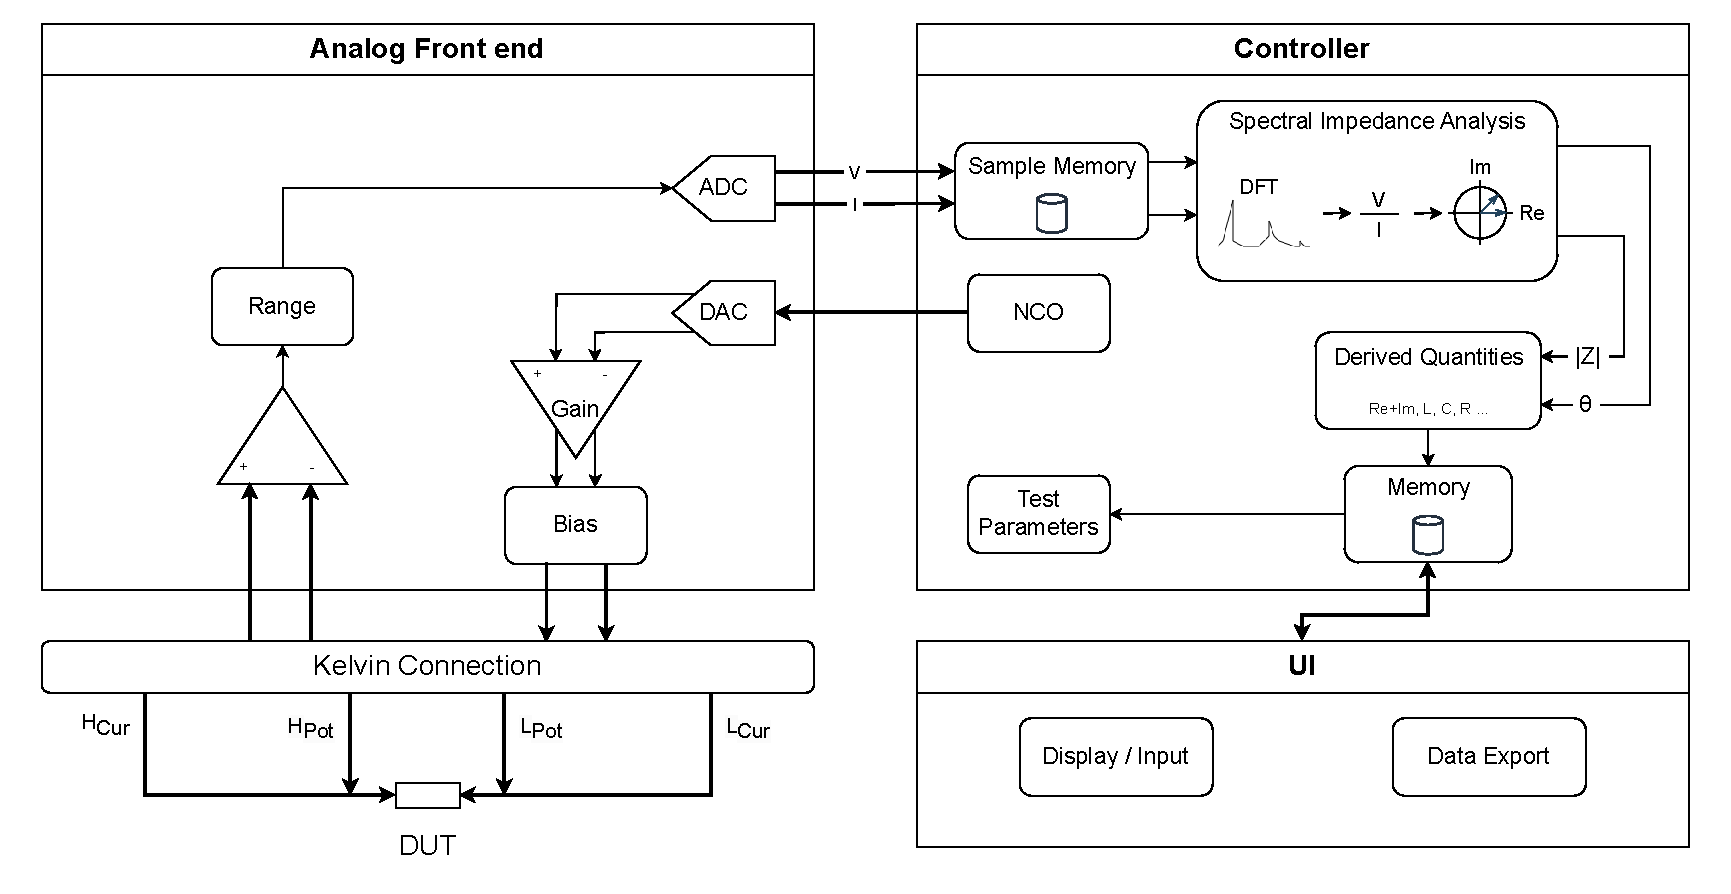
\includegraphics[width=1\textwidth]{Sections/6_SystemArchitecture/Figures/SystemArchitecture.pdf}
    \caption{The proposed system architecture for the impedance analyzer designed in this document. An analog front end will measure DUT voltage and current, 
    this will then undergo spectral analysis, such that phase and magnitude information can be obtained and used to calculate all derived quantities. A user can set the test parameters using a UI, these parameters in turn will determine DAC settings, range and sample rate.}
    \label{fig_6_SysArchitecture}
\end{figure}